\documentclass{assignment}
\usepackage[utf8]{inputenc}
\usepackage[T1]{fontenc}
\usepackage{hyperref}
\usepackage{listings}

%\lstset{
%	inputencoding=utf8,
%	literate=
%	{á}{{\'a}}1
%	{é}{{\'e}}1
%	{í}{{\'i}}1
%	{ó}{{\'o}}1
%	{ú}{{\'u}}1
%	{Á}{{\'A}}1
%	{É}{{\'E}}1
%	{Í}{{\'I}}1
%	{Ó}{{\'O}}1
%	{Ú}{{\'U}}1
%	{ñ}{{\~n}}1
%	{Ñ}{{\~N}}1
%}
%
%
%\lstdefinelanguage{Pseudocodigo}{
%	morekeywords={
%		SI, ENTONCES, SINO, FIN, MIENTRAS, HACER, PARA, DESDE, HASTA,
%		FUNCIÓN, PROCEDIMIENTO, CLASE, CONSTRUCTOR, ATRIBUTOS,
%		RETORNAR, ALGORITMO, CONSTANTE, NUEVO, Y, O, NO, CADA, EN
%	},
%	sensitive=false,
%	morecomment=[l]{//},
%	morestring=[b]",
%}
%
%\lstset{
%	language=Pseudocodigo,
%	basicstyle=\ttfamily\small,
%	keywordstyle=\color{blue}\bfseries,
%	commentstyle=\color{gray}\itshape,
%	stringstyle=\color{orange},
%	numbers=left,
%	numberstyle=\tiny\color{gray},
%	stepnumber=1,
%	breaklines=true,
%	frame=single,
%	tabsize=4,
%	showstringspaces=false,
%}
\begin{document}
	
	\assignmentTitle{Claudio Iván Esparza Castañeda}{Luis Alberto Balam Guzmán}{./Logo.png}{Maestría en Sistemas Embebidos}{Programación y Procesamiento de Datos}{5A. Práctica de hilos en Python}
	\section*{Objetivo}
	Lo que hizo Arduino por la cultura maker fue fundamental para democratizar la tecnología. Por otro lado, otro impulso se dio a través del uso de Python por la misma comunidad (junto a su creador, Guido Van Rossum). En algún punto estas dos fuerzas convergieron para llegar a micropython, que es un proyecto que empuja hacia esta democratización para el tipo de usuario que en su día a día no tiene tiempo de aprender todo acerca del hardware, pero busca realizar proyectos de fin de semana, o bien el profesional o el estudiante que requiere un prototipado rápido para el proyecto de fin de semana. Después del Arduino, han aparecido diferentes soluciones con distintos controladores. Así es como llegamos a la Raspberry Pi Pico, que se puede programar a través de bare-metal, con RTOS (FreeRTOS, Zephyr, etc.), o micropython.\\
	Con la imposibilidad que representa tener que procesar grandes cantidades de información en un medio con pocos recursos, refiriéndonos en este caso a la Raspberry Pi Pico, surge la necesidad de contar con sistemas híbridos: control en el sistema embebido, y procesamiento en la computadora.\\
	En sistemas modernos, se cuenta con controladores y procesadores con múltiples núcleos. Eso, además de arquitecturas basadas en pipeline permiten manejar múltiples operaciones en un solo chip, empleando distintas operaciones.
	\section*{Descipción de la solución}
	Se sigue la estructura propuesta para el proyecto. Hay un único cambio realizado en el archivo {\tt generador\_senial.py} fue renombrarlo a {\tt main.py} e incluirlo en la carpeta {\tt pico}$\slash$, Este cambio se realizó con el objetivo de poder usar el puerto serial sin que se bloqueé el puerto serial por el REPL.\\
	Por otro lado, se dividieron responsabilidades a través de las distintas partes requeridas. Por un lado, el archivo {\tt adquisicion.py} contiene la información relacionada al primer hilo. El archivo {\tt procesamiento.py} se encuentra el segundo hilo, donde se realiza el procesamiento  de la señal. Por último, el archivo {\tt registro.py} contiene el tercer hilo, y guarda el log en un csv.\\
	Se sigue usando el archivo {\tt funciones.py} de tareas anteriores, con el objetivo de hacer algunas validaciones. El archivo {\tt main.py} se encarga de ejecutar todo lo anterior en el orden dado.
	\section*{Metodología}
	El tratamiento de las señales se realiza con SciPy, al emplear las funciones definidas en este módulo. Se emplea SciPy para calcular los valores para el procesamiento de señal, como el RMS, promedio, desviación estándar.\\
	Se emplea Serial Studio para el análisis de la transmisión serial con la tarjeta. Posteriormente se trabaja para codificar la comunicaicón en el programa de python.
	\section*{Capturas de ejecución}
	\begin{figure}[htbp]
		\centering
		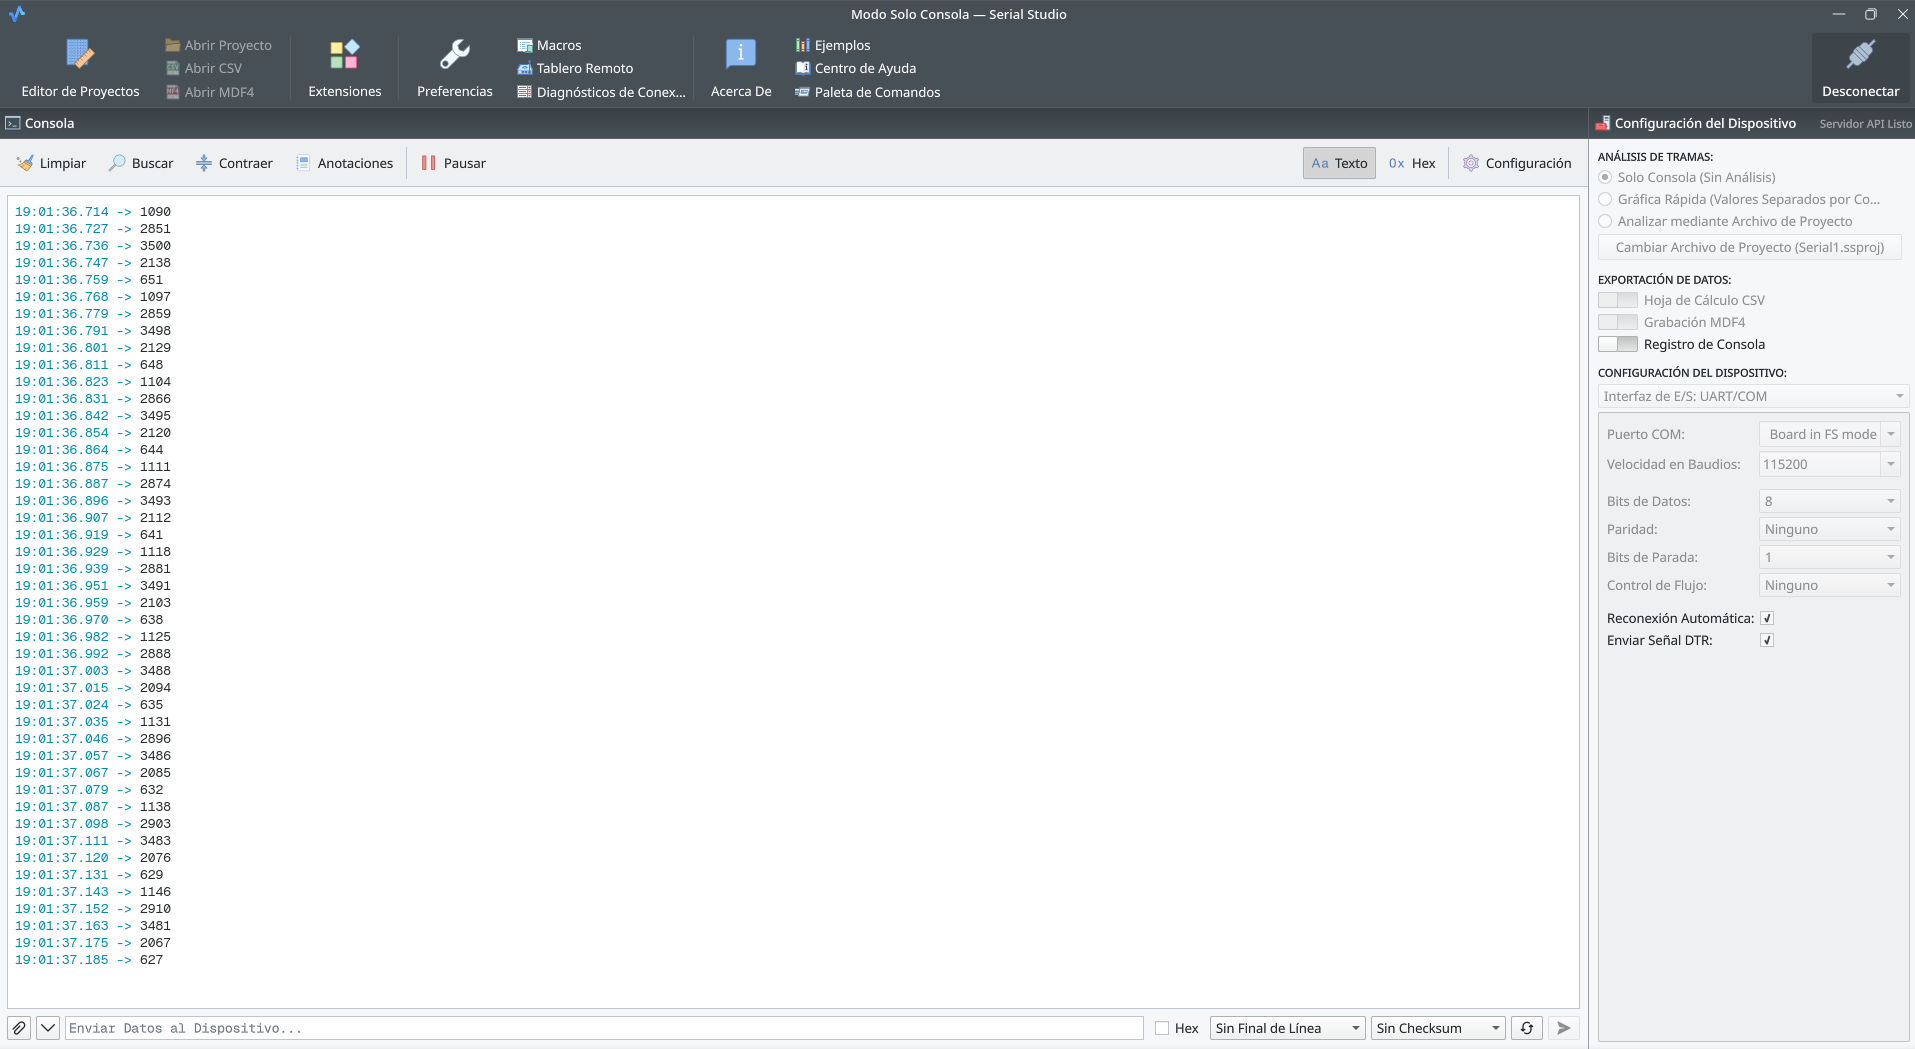
\includegraphics[width=\textwidth]{Figuras/1}
		\caption{Serial studio con la transmisión serial}
		\label{fig:1}
	\end{figure}
	\begin{figure}[htbp]
		\centering
		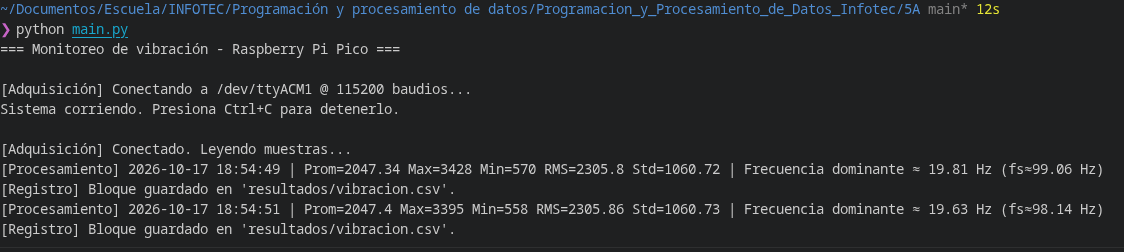
\includegraphics[width=\textwidth]{Figuras/2}
		\caption{Inicio de ejecución}
		\label{fig:2}
	\end{figure}
	\begin{figure}[htbp]
		\centering
		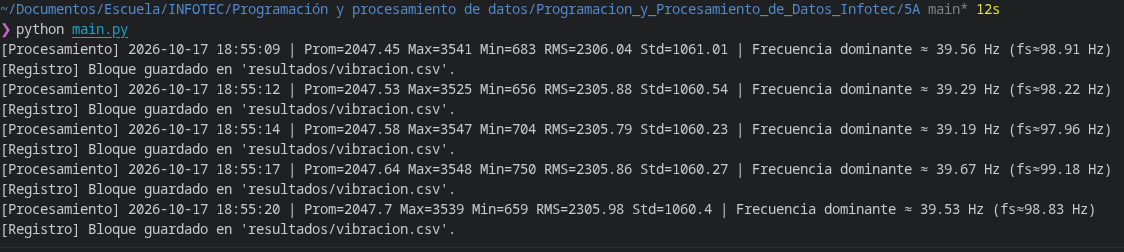
\includegraphics[width=\textwidth]{Figuras/3}
		\caption{Ejecución contínua}
		\label{fig:3}
	\end{figure}
	\begin{figure}[htbp]
		\centering
		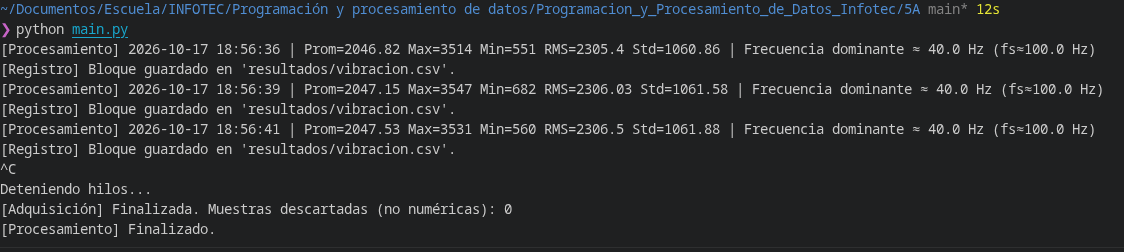
\includegraphics[width=\textwidth]{Figuras/4}
		\caption{Ejecución contínua}
		\label{fig:4}
	\end{figure}
	\begin{figure}[htbp]
		\centering
		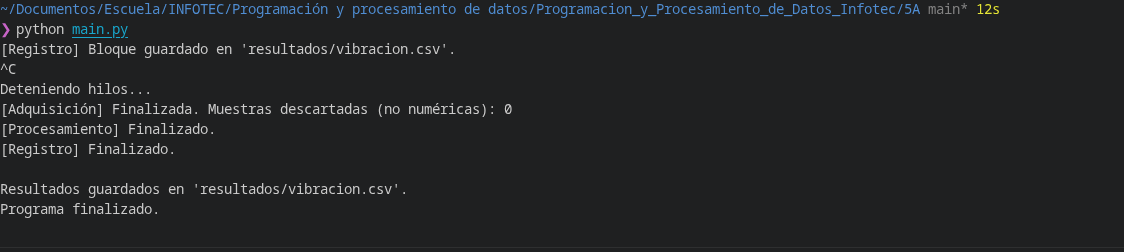
\includegraphics[width=\textwidth]{Figuras/5}
		\caption{Corte de la ejecución del programa}
		\label{fig:5}
	\end{figure}
	\section*{Conclusiones}
	\begin{itemize}
		\item {\bf ¿Qué problema se presentaría si todo fuera presencial?} El programa tendría que leer, procesar y duardar en ese orden, y mientras hace una cosa no puede hacer las otras. El retardo provocaría el bloqueo del puerto serial.
		\item {\bf ¿Qué ventajas aportan los hilos en adquisión de datos?} La existencia de la concurrencia real de tareas permite que la lectura no se detenga. Permiten aprovechar los tiempos de espera que existen entre la lectura serial y la escritura a disco, pues ambas son operaciones de entrada y salida. Permite aguardar el Ctrl+C mientras trabaja.
		\item {\bf ¿Por qué separar adquisión y procesamiento?} La  adquisión debe ocurrir al ritmo del sensor. El procesamiento es de tiempo flexible, lo que puede tardar más o menos según la carga. Si ambos van juntos, el más lento dicta el ritmo del otro.
		\item {\bf ¿En qué aplicaciones reales se usan arquitecturas similares?} Monitoreo de entorno industriales, automotriz que incorpora la adquisión de de sensores separada del procesamiento y la comunicación. Telemetría y robótica, entre otras aplicaciones.
	\end{itemize}
	La carpeta en el repositorio de este proyecto es: \href{https://github.com/clivan/Programacion_y_Procesamiento_de_Datos_Infotec/5A}{Programación y procesamiento de Datos}.	
\end{document}
